% !TEX TS-program = pdflatex
% !TEX encoding = UTF-8 Unicode

% This file is a template using the "beamer" package to create slides for a talk or presentation
% - Talk at a conference/colloquium.
% - Talk length is about 20min.
% - Style is ornate.

% MODIFIED by Jonathan Kew, 2008-07-06
% The header comments and encoding in this file were modified for inclusion with TeXworks.
% The content is otherwise unchanged from the original distributed with the beamer package.

\documentclass{beamer}


% Copyright 2004 by Till Tantau <tantau@users.sourceforge.net>.
%
% In principle, this file can be redistributed and/or modified under
% the terms of the GNU Public License, version 2.
%
% However, this file is supposed to be a template to be modified
% for your own needs. For this reason, if you use this file as a
% template and not specifically distribute it as part of a another
% package/program, I grant the extra permission to freely copy and
% modify this file as you see fit and even to delete this copyright
% notice. 


\mode<presentation>
{
  \usetheme{Warsaw}
  % or ...

  \setbeamercovered{transparent}
  % or whatever (possibly just delete it)
}


\usepackage[english]{babel}
% or whatever

\usepackage[utf8]{inputenc}
% or whatever

\usepackage{times}
\usepackage{overpic}
\usepackage[T1]{fontenc}
% Or whatever. Note that the encoding and the font should match. If T1
% does not look nice, try deleting the line with the fontenc.


\title[SVD Image Compression] % (optional, use only with long paper titles)
{Image Compression via Singular Value Decomposition}


\author[Matt Mastin]% (optional, use only with lots of authors)
{Matt Mastin\inst{}}
% - Give the names in the same order as the appear in the paper.
% - Use the \inst{?} command only if the authors have different
%   affiliation.

\institute[Universities of Somewhere and Elsewhere] % (optional, but mostly needed)
{
  \inst{}%
  Data Software Engineer\\
  MailChimp
  }
% - Use the \inst command only if there are several affiliations.
% - Keep it simple, no one is interested in your street address.





% If you have a file called "university-logo-filename.xxx", where xxx
% is a graphic format that can be processed by latex or pdflatex,
% resp., then you can add a logo as follows:

% \pgfdeclareimage[height=0.5cm]{university-logo}{university-logo-filename}
% \logo{\pgfuseimage{university-logo}}



% Delete this, if you do not want the table of contents to pop up at
% the beginning of each subsection:
\AtBeginSection[]
{
  \begin{frame}<beamer>{Outline}
    \tableofcontents[currentsection,currentsubsection]
  \end{frame}
}


% If you wish to uncover everything in a step-wise fashion, uncomment
% the following command: 

%\beamerdefaultoverlayspecification{<+->}


\begin{document}

\begin{frame}
  \titlepage
\end{frame}

\begin{frame}{Outline}
  \tableofcontents
  % You might wish to add the option [pausesections]
\end{frame}


% Structuring a talk is a difficult task and the following structure
% may not be suitable. Here are some rules that apply for this
% solution: 

% - Exactly two or three sections (other than the summary).
% - At *most* three subsections per section.
% - Talk about 30s to 2min per frame. So there should be between about
%   15 and 30 frames, all told.

% - A conference audience is likely to know very little of what you
%   are going to talk about. So *simplify*!
% - In a 20min talk, getting the main ideas across is hard
%   enough. Leave out details, even if it means being less precise than
%   you think necessary.
% - If you omit details that are vital to the proof/implementation,
%   just say so once. Everybody will be happy with that.



\section{Singular Value Decomposition}

\begin{frame}{Images are Matrices}
\begin{itemize}

\item An image can be viewed as a matrix where each entry in the matrix represents a pixel.

	\begin{itemize}
	\item If we greyscale the image the entries are just numbers!
	\item (otherwise they would be something like triples representing RGB values)
	\end{itemize}

\item So, we can apply techniques from linear algebra to manipluate images!

\end{itemize}  
\end{frame}

\begin{frame}{Some Linear Algebra}
\begin{itemize}

\item Given a matrix $M$ we can decompose it as $M = U~\Sigma~V$ where $U$, $\Sigma$, and $V$ have some nice properties.

\item $\Sigma$ is matrix whose non-zero entries are located on the main diagonal and these values contain information about how the columns of $U$ relate to the matrix $M$.

\end{itemize}  
\end{frame}

\begin{frame}{Schematic Example}
\begin{center}
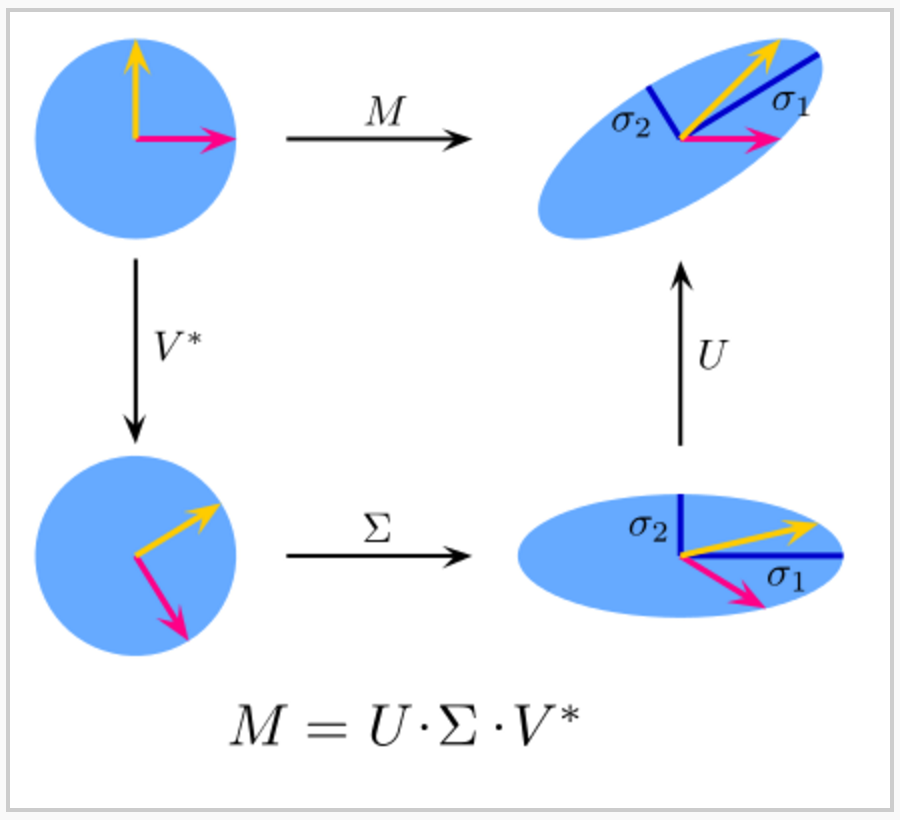
\includegraphics[width=7cm]{svd.png}
\end{center}
\end{frame}

\begin{frame}{Some Linear Algebra}
\begin{itemize}

\item The columns of $U$ whose corresponding values in $\Sigma$ (called singular values) are large can be interpreted as the ``most important'' in relation to $A$.

\item In a sense we can approximate $A$ by only paying attention to the first $N$ ``most important'' columns of $U$.

\end{itemize}  
\end{frame}

\section{Application to Image Compression}

\begin{frame}{The Big Picture}

\begin{center}
\begin{overpic}[width=8.5cm]{subspace.png}
\put(5,5){{\small Subspace of compressible images}}
\put(70,67){{\small Original image}}
\put(71,55){{\small Decompressed}}
\put(85,50){{\small image}}
\end{overpic}

\end{center}

\end{frame}

\begin{frame}{Where's the Compression?}

\begin{itemize}
\item The original image can be described with two coordinates.

\item The compressed can be described with only one coordinate: the distance along the line from the origin!

\item So, we have halved the amount of information needed to store the image.

\end{itemize}

\end{frame}

\begin{frame}{This is Really Least Squares (Some Math)}

\begin{center}
\begin{overpic}[width=5cm]{subspace.png}
\put(11,3){{\small Col($A$)}}
\put(70,67){{\small $b$}}
\put(85,53){{\small $\hat{b}$}}
\end{overpic}

\end{center}

\begin{itemize}
\item If $A$ is the matrix of ``important'' columns of the image matrix $M$, then the equation $Ax=b$ has a solution if $b$ is in the span of the columns of $A$. 
\end{itemize}

\end{frame}

\begin{frame}{This is Really Least Squares (Some Math)}

\begin{center}
\begin{overpic}[width=5cm]{subspace.png}
\put(11,3){{\small Col($A$)}}
\put(70,67){{\small $b$}}
\put(85,53){{\small $\hat{b}$}}
\end{overpic}

\end{center}

\begin{itemize}
\item But here, $b$ is not in the column space of $A$, so we do the best we can: project $b$ into $Col(A)$ and solve the equation $Ax=\hat{b}$ which DOES have a solution.
\end{itemize}

\end{frame}

\begin{frame}{This is Really Least Squares (Some Math)}

\begin{center}
\begin{overpic}[width=5cm]{subspace.png}
\put(11,3){{\small Col($A$)}}
\put(70,67){{\small $b$}}
\put(85,53){{\small $\hat{b}$}}
\end{overpic}

\end{center}

\begin{itemize}
\item A solution to $Ax=\hat{b}$ is a compressed representation of the image $b$ and we recover the decompressed image $\hat{b}$ by multiplying by $A$.
\end{itemize}

\end{frame}

\section{The Code}


\section{Examples}

\begin{frame}{Cards on the Table}

\begin{itemize}
\item I had trouble working with large images in sklearn due to what seem to be memory issues related to blocking high resolution images. 

\item The following is a low resolution example generated in python.
\end{itemize}

\end{frame}

\begin{frame}{Cards on the Table}

{\large The following examples were generated using the same algorithm, but implemented in Mathematica.}

\end{frame}

\begin{frame}{I Like Dogs}
\begin{center}
\includegraphics[width=4.5cm]{dog_2.jpg}
\end{center}
\end{frame}

\begin{frame}{Compressed $90\%$}
\begin{center}
\includegraphics[width=4.5cm]{matt90dog_2.jpg}
\end{center}
\end{frame}

\begin{frame}{Compressed $99\%$}
\begin{center}
\includegraphics[width=4.5cm]{matt99dog_2.jpg}
\end{center}
\end{frame}

\begin{frame}{I Like Dogs}
\begin{center}
\includegraphics[width=4.5cm]{dog_6.jpg}
\end{center}
\end{frame}

\begin{frame}{Compressed $90\%$}
\begin{center}
\includegraphics[width=4.5cm]{matt90dog_6.jpg}
\end{center}
\end{frame}

\begin{frame}{Compressed $99\%$}
\begin{center}
\includegraphics[width=4.5cm]{matt99dog_6.jpg}
\end{center}
\end{frame}

\begin{frame}{I Like Dogs}
\begin{center}
\includegraphics[width=8cm]{dog_9.jpg}
\end{center}
\end{frame}

\begin{frame}{Compressed $90\%$}
\begin{center}
\includegraphics[width=8cm]{matt90dog_9.jpg}
\end{center}
\end{frame}

\begin{frame}{Compressed $99\%$}
\begin{center}
\includegraphics[width=8cm]{matt99dog_9.jpg}
\end{center}
\end{frame}

\begin{frame}{I Like Dogs}
\begin{center}
\includegraphics[width=8cm]{dog_17.jpg}
\end{center}
\end{frame}

\begin{frame}{Compressed $90\%$}
\begin{center}
\includegraphics[width=8cm]{matt90dog_17.jpg}
\end{center}
\end{frame}

\begin{frame}{Compressed $99\%$}
\begin{center}
\includegraphics[width=8cm]{matt99dog_17.jpg}
\end{center}
\end{frame}


\end{document}


